\chapter{Teknik \textit{Dynamic Programming}}\label{ch:modul5}

\section{Pengenalan \textit{Dynamic Programming}}
\textit{Dynamic programming} merupakan pendekatan lain dalam memecahkan permasalahan seperti pendekatan \textit{divide and conguer}. Kata \textit{programming} di nama \textit{dynamic programming} tidak berhubungan dengan menulis kode komputer melainkan lebih ke arah metode tabular (kata \textit{dynamic programming} sebenarnya dipopulerkan di bidang matematika bukan ilmu komputer/teknik informatika).

Di \textit{divide and conguer}, permasalahan dipecah menjadi sub-permasalahan yang lebih kecil kemudian dipecahkan secara terpisah dan akhirnya digabungkan. Kelemahan dalam pendekatan ini adalah, beberapa sub-permasalahan sebenarnya memiliki solusi pemecahan yang sama akan tetapi di \textit{divide and conguer} hal itu tidak diperdulikan, melainkan sub-permasalahan yang sama akan diselesaikan berkali-kali sehingga mengakibatkan pemborosan sumber daya komputasional.

Di \textit{dynamic programming} sub-permasalahan yang sama hanya dipecahkan sekali saja dan disimpan solusinya ke dalam tabel (itu sebabnya ia disebut sebagai metode tabular). Apabila ditemukan sub-permasalahan yang sama kelak, maka solusi yang telah disimpan akan dipergunakan kembali.

\textit{Dynamic programming} sering dipakai untuk menyelesaikan permasalahan yang bersifat optimisasi. Permasalahan tersebut mempunyai berbagai macam solusi, akan tetapi hanya ada satu yang nilainya optimal (misalnya nilai paling maksimal atau minimal). Nilai yang paling optimal tersebut disebut juga sebagai solusi optimal dari suatu permasalahan.

Terdapat 4 langkah dalam penyelesaian permasalahan \textit{dynamic programming}:
\begin{enumerate}
	\item Gambarkan struktur dari solusi optimal.
	\item Definisikan nilai dari solusi optimal secara rekursif.
	\item Hitung nilai dari solusi optimal.
	\item Bentuk solusi optimal dari informasi yang sudah dihitung sebelumnya.
\end{enumerate}

\section{Dynamic Programming, Sub-Permasalahan, dan Memoization}

Mari kita mulai penjelasan DP dengan contoh yang paling sederhana terlebih dahulu: perhitungan bilangan fibonacci. Algoritma~\ref{algo:fibonacci-recurse} menunjukkan algoritma perhitungan bilangan fibonacci yang sederhana.

\lstinputlisting[language=Python, 
                 label={algo:fibonacci-recurse},
                 linebackgroundcolor={\ifnum\value{lstnumber}=5\color{codehighlight}\fi},
                 caption=Algoritma Fibonacci Rekursif
                ]
                {code/9-fibonacci.py}

Pada baris ke 5 Algoritma~\ref{algo:fibonacci-recurse} kita dapat melihat bagaimana untuk menyelesaikan perhitungan fibonacci, kita menghitung dua bilangan fibonacci sebelumnya dengan fungsi yang sama (rekursif). Kita dapat menanggap bagian ini sebagai pemecahan masalah ke sub-permasalahan, di mana:

\begin{itemize}
    \item Permasalahan utama kita adalah perhitungan bilangan fibonacci ke $n$, dan
    \item sub-permasalahan adalah menghitung bilangan fibonacci yang lebih kecil ($n - 1$ dan $n - 2$).
\end{itemize}

Kita dapat melihat bagaimana jalur kalkulasi rekursif dari Algoritma~\ref{algo:fibonacci-recurse} pada Gambar~\ref{fig:fibonacci-recurse}.

\begin{figure}
    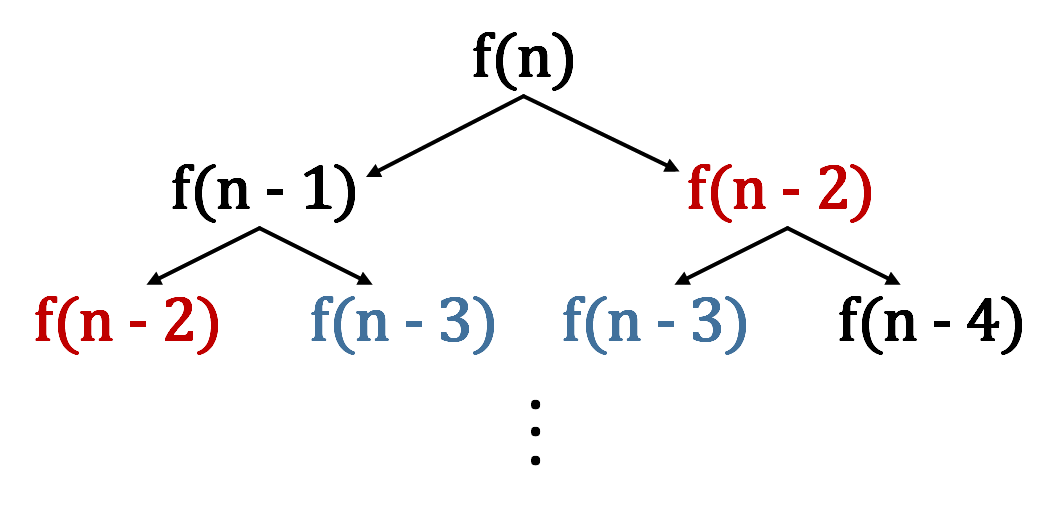
\includegraphics[width=\textwidth,keepaspectratio]{fig/FibonacciCallStack.png}%
	\caption{Proses Pemanggilan Fibonacci}%
	\label{fig:fibonacci-recurse}%
\end{figure}

Pada Gambar~\ref{fig:fibonacci-recurse} kita dapat melihat bagaimana terdapat beberapa fungsi yang perhitungannya kita lakukan beberapa kali, yaitu $f(n - 2)$ dan $f(n - 3)$. Jika perhitungan ini terus diturunkan, kita akan melihat terdapat banyak duplikasi perhitungan seperti ini sampai kita selesai melakukan rekursi. Semakin dalam penurunan fungsi rekursifnya, semakin banyak pula perhitungan kembali yang harus kita lakukan. Karena perhitungan yang dilakukan berulang kali ini, pada dasarnya kita menjalankan $2^n$ langkah pada setiap pemanggilan fungsi fibonacci. Kompleksitas $O(2^n)$ ini tentu saja sangat, sangat buruk.

\marginnote[-4cm]{
    \begin{latihan}
        Bagaimana kita dapat mengetahui bahwa Algoritma~\ref{algo:fibonacci-recurse} memiliki kompleksitas $O(2^n)$? Turunkan perhitungannya!
    \end{latihan}
}

Untuk mengurangi perulangan perhitungan ini, kita dapat menyimpan hasil perhitungan fungsi yang telah kita lakukan sebelumya, seperti yang tampak pada Algoritma~\ref{algo:fibonacci-memoization}.

\lstinputlisting[language=Python, 
                 label={algo:fibonacci-memoization},
                 caption=Algoritma Fibonacci dengan Penyimpanan Hasil,
                 float=t
                ]
                {code/10-fibonacci-memoized.py}

Pada Algoritma~\ref{algo:fibonacci-memoization}, kita dapat melihat bagaimana penyimpanan hasil kalkulasi dilakukan dengan \textit{dictionary}. Pada prakteknya, kita dapat menggunakan struktur data apapun, sesuai dengan kebutuhan kita. Penyimpanan hasil kalkulasi ini akan dapat mengurangi jumlah pemanggilan rekursif yang harus kita lakukan, menjadi seperti pada Gambar~\ref{fig:fibonacci-memoization} saja.

\begin{figure}
    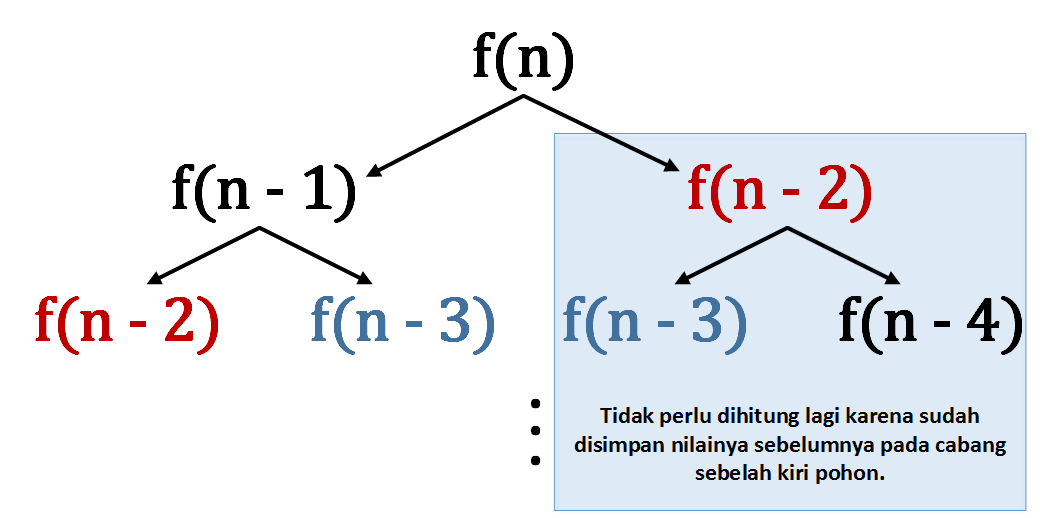
\includegraphics[width=\textwidth,keepaspectratio]{fig/FibonacciDPCallStack.png}%
	\caption{Proses Pemanggilan Fibonacci dengan Penyimpanan Hasil}%
	\label{fig:fibonacci-memoization}%
\end{figure}

Teknik menyimpan hasil kalkulasi agar tidak perlu melakukan perhitungan yang sama berulang kali ini kita kenal dengan nama \textbf{memoization}. Sampai titik ini, kita dapat dikatakan telah menggunakan tekik \textit{dynamic programming} untuk melakukan perhitungan fibonacci. Perhitungan sub-masalah dilakukan secara \textit{lazy} pada Algoritma~\ref{algo:fibonacci-memoization}, karena perhitungan baru dilakukan ketika diperlukan.

Karena banyak sub-masalah yang kita selesaikan melalui memo pada Algoritma~\ref{algo:fibonacci-memoization}, jumlah langkah yang diperlukan untuk menyelesaikan algoritma berkurang menjadi $O(n)$ saja. Kompleksitas $O(1)$ ini didapatkan dengan mengasumsikan pemanggilan isi memori dapat kita anggap sebagai $O(1)$. Pada dasarnya di Algoritma~\ref{algo:fibonacci-memoization} kita melakukan pertukaran jumlah langkah eksekusi dengan memori.

Meskipun telah meningkatkan kompleksitas dengan sangat baik, pada prakteknya Algoritma~\ref{algo:fibonacci-memoization} masih memiliki kekurangan, yaitu penggunaan \textit{stack space} yang terlalu besar. Pada bahasa yang memiliki batasan ukuran stack dan kedalaman rekursif seperti python, hal ini dapat menjadi masalah tersendiri. Untuk menanggulangi hal ini, kita dapat menggunakan pendekatan selain \textit{lazy} pada \textit{dynamic programming}, yaitu pendekatan \textit{bottom-up}.

Algoritma~\ref{algo:fibonacci-bottom-up} menunjukkan cara perhitungan fibonacci secara \textit{bottom-up}.

\lstinputlisting[language=Python, 
                 label={algo:fibonacci-bottom-up},
                 caption=Algoritma Fibonacci Bottom-Up
                ]
                {code/11-fiibonacci-bottom-up.py}

Pada teknik \textit{bottom-up} yang digunakan dalam Algoritma~\ref{algo:fibonacci-bottom-up}, kita terlebih dahulu menentukan urutan operasi yang akan dilakukan. Sebelum mulai melakukan perhitungan, kita mengetahui beberapa hal:

\begin{itemize}
    \item Semua hasil kalkulasi disimpan dalam $memo$.
    \item Pada fibonacci tradisional, kita akan menghitung nilai fibonacci dari $n$ sampai $1$,
    \item bilangan fibonacci selalu membutuhkan dua buah bilangan fibonacci sebelumnya.
    \item Urutan kalkulasi yang dilakukan pada fibonacci tradisional adalah $f(n)$, $f(n - 1)$, $f(n -2)$, dst.
\end{itemize}

Pada pendekatan \textit{bottom-up}, kita hanya semata-mata mengganti urutan operasi dari fibonacci. Karena kita tahu perhitungan fibonacci ke $n$ akan memerlukan perhitungan fibonacci ke $1$ sampai $n$, kita dapat melakukan perhitungan tersebut secara langsung (dari $1$ sampai $n$; kecil ke besar; \textit{bottom-up}) alih-alih menghitung dari $n$ sampai ke $1$ (besar ke kecil; \textit{top-down}) yang apda setiap langkahnya kita harus menunggu hasil perhitungan baru. Perhatikan juga bagaimana inti algoritma (bagian $if n <= 2$) pada Algoritma~\ref{algo:fibonacci-recurse}, ~\ref{algo:fibonacci-memoization}, dan ~\ref{algo:fibonacci-bottom-up} adalah sama. Hal ini menunjukkan bagaimana pada dasarnya kita melakukan perhitungan yang sama, dengan metode yang berbeda dan lebih efisien.

Sampai titik ini kita telah melihat bagian paling mendasar dari \textit{dynamic programming}, yaitu pemecahan sub-masalah dan \textit{memoization}. Bagian lain yang tak kalah pentingnya dari \textit{dynamic programming} adalah optimasi. Mari kita lihat contoh lain yang akan memberikan kita langkah optimasi pada \textit{dynamic programming}.

\section{Optimasi}

Kegunaan utama dari DP adalah untuk menyelesaikan masalah \textbf{optimasi}. Permasalahan optimasi artinya permasalahan yang mencari nilai \textbf{terbaik}, baik maksimal maupun minimal, dari sebuah solusi. Salah satu contoh paling praktis dalam penerapan DP model ini adalah algoritma untuk membuat teks rata tengah. Bagaimana cara kerja algoritma ini? Mari kita lihat masalah yang ingin diselesaikan terlebih dahulu.

Pada aplikasi pengolah kata seperti Microsoft Word, biasanya terdapat fitur untuk menentukan kemerataan teks yang ada pada paragraf, seperti yang nampak pada Gambar~\ref{fig:text-align}.

\begin{figure}
    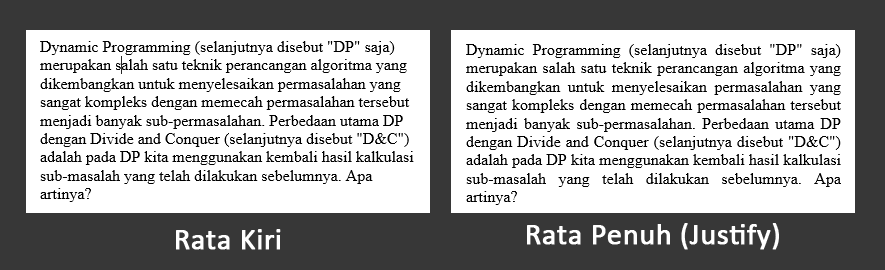
\includegraphics[width=\textwidth,keepaspectratio]{fig/TextAlign}
	\caption{Pemerataan Teks pada Microsoft Word}
	\label{fig:text-align}
\end{figure}

Bagaimana kita menentukan kemerataan teks? Secara umum, kemerataan sebuah teks ditentukan oleh beberapa hal berikut:

\begin{enumerate}
    \item Ukuran dari halaman, yang tentunya akan mempengaruhi berapa lebar maksimal dari sebuah teks.
    \item Ukuran setiap kata yang ada dalam teks, untuk menghitung berapa banyak kata yang dapat dimasukkan ke dalam satu baris teks.
    \item Ukuran spasi dalam teks, seperti ukuran kata, untuk menghitung jumlah kata yang dapat dimasukkan ke dalam teks.
    \item Ukuran karakter-karakter khusus seperti "!", "?", ",",".", dan lainnya. Meskipun biasanya berukuran kecil, karakter khusus tetap berperan dalam mengisi ruang tulisan.
\end{enumerate}

Dengan melakukan kalkulasi sederhana dari teks, tentunya kita bisa saja melakukan pemerataan teks dengan mudah. Misalnya, untuk menghitung total teks yang dapat masuk ke dalam sebuah baris tulisan, kita dapat menggunakan Persamaan~\ref{eq:total-teks-per-baris}.

\begin{equation}\label{eq:total-teks-per-baris}
    \text{ukuran halaman} \gets \text{total ukuran kata} + \text{total ukuran spasi} + \text{total ukuran simbol}
\end{equation}

Sehingga untuk membuat sebuah teks menjadi rata penuh (\textit{justified}) kita dapat memasukkan setiap kata, spasi, dan simbol satu demi satu sampai kita memenuhi sebuah baris. Jika kata selanjutnya tidak lagi memiliki ukuran yang cukup, maka kita dapat menambahkan spasi di tengah-tengah kata sebelumnya sampai baris penuh, dan lalu berpindah baris.

Secara sederhana, algoritma naif untuk melakukan rata penuh teks adalah seperti berikut:

\begin{enumerate}
    \item Ambil satu elemen dalam teks, baik berupa kata, simbol, maupun spasi. Masukkan elemen ini ke dalam baris.
    \item Hitung ukuran baris sekarang.
    \item Ambil satu elemen lagi dalam teks, dan hitung ukurannya.
    \item Tambahkan ukuran baris sekarang dengan ukuran elemen berikutnya. Hasil pengukuran ini selanjutnya akan disebut "Ukuran Baris Selanjutnya" atau UBS.
    \item Cek nilai UBS:
        \begin{enumerate}
            \item Jika UBS masih lebih kecil dari lebar halaman, kembali ke langkah 1
            \item Jika UBS sudah lebih dari lebar halaman:
                \begin{enumerate}
                    \item Tambahkan spasi di antara setiap kata dalam baris sampai ukuran baris sama dengan lebar halaman.
                \end{enumerate}
        \end{enumerate}
\end{enumerate}

Dalam bentuk lebih formalnya, Algoritma~\ref{algo:text-justification-raw} menjukkan contoh implementasi sederhana pemerataan teks (berbeda dengan algoritma lain sebelumnya, algoritma ini tidak dapat dijalankan dan digunakan hanya sebagai ilustrasi).

\lstinputlisting[language=Python, 
                 label={algo:text-justification-raw},
                 caption=Algoritma Naif Pemerataan Teks
                ]
                {code/12-text-justification-raw.py}

Hasil Algoritma~\ref{algo:text-justification-raw} kurang optimal, karena ketika terdapat kata-kata yang panjang dalam sebuah kalimat, kita terpaksa harus memotong baris terlalu cepat, dan akhirnya menambahkan banyak spasi. Contoh eksekusi dari algoritma di atas dapat dilihat pada gambar berikut:

\begin{figure}
    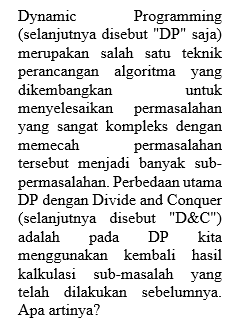
\includegraphics{fig/TextAlignJustify-Greedy-Bad}
	\caption{Hasil Algoritma Pemerataan Teks Sederhana}
	\label{fig:text-align-raw}
\end{figure}

Perhatikan bagaimana teks "Dynamic Programming", "dikembangkan untuk", dan "memecah permasalahan" memiliki spasi yang sangat lebar. Menggunakan DP, kita dapat menghasilkan pemerataan teks yang lebih optimal.

Berdasarkan algoritma sebelumnya yang kita kembangkan, dapat dilihat bagaimana optimasi dari rata penuh sebuah teks terdapat pada \textbf{kapan kita melakukan pergantian baris}. Jika kita mengganti baris terlalu cepat (jumlah kata masih sedikit), maka secara otomatis kita harus menambahkan banyak spasi, yang menyebabkan teks tidak enak dilihat. Untuk mendapatkan jumlah kata yang optimal dalam sebuah baris, kita akan melakukan perhitungan tingkat "keburukan" sebuah kata dalam teks, jika kata tersebut dijadikan pengganti baris. Kita kemudian dapat mencari tingkat keburukan setiap kata yang ada dalam teks, dan mengambil kata yang memiliki tingkat keburukan terendah sebagai tanda berganti baris.

Pengukuran tingkat keburukan teks sendiri tentunya ditentukan oleh jumlah ruang kosong yang ada dari teks sampai ke ujung halaman. Misalnya, pada Gambar~\ref{fig:text-align-badness} kita dapat melihat contoh ruang kosong dari teks sampai ke ujung halaman.

\begin{figure}
    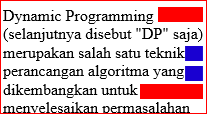
\includegraphics{fig/TextAlign-Badness}
	\caption{Tingkat Keburukan Teks}
	\label{fig:text-align-badness}
\end{figure}

Pada gambar di atas, blok berwarna merah berarti tingkat keburukannya tinggi, dan blok berwarna hijau berarti tingkat kebukurannya rendah. Untuk mendapatkan nilai keburukan yang paling kecil dalam sebuah teks, tentunya kita harus menghitung seluruh kombinasi nilai keburukan dari elemen-elemen yang ada dalam teks. Perhitungan kombinasi nilai keburukan ini tentunya merupakan masalah yang tepat untuk algoritma DP, karena setiap perhitungan nilai keburukan pada dasarnya adalah sebuah sub-masalah!

Jadi sekarang kita telah menemukan sub-masalahnya: mencari nilai keburukan dari sebuah elemen. Bagaimanakah kita dapat menggunakan teknik DP untuk menyelesaikan masalah ini? Ketika menghitung kombinasi dari nilai keburukan dari setiap elemen, secara tidak langsung kita akan membangun sebuah Directed Acyclic Graph, seperti yang tampak pada Gambar~\ref{fig:dag-in-text}.

\begin{figure}
    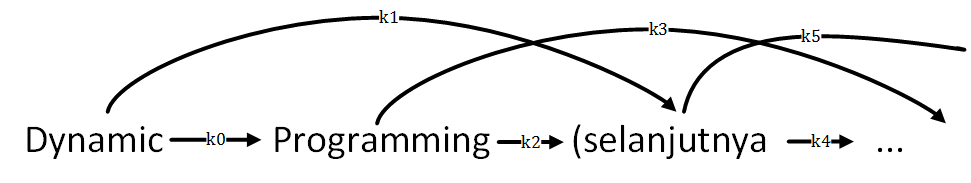
\includegraphics[width=\textwidth,keepaspectratio]{fig/TextAlign-DAG}
	\caption{DAG dalam Teks}
	\label{fig:dag-in-text}
\end{figure}

dengan setiap $k$ merepresentasikan tingkat keburukan dari elemen tersebut. Menggunakan informasi tersebut, kita dapat mencari nilai minimal dari total seluruh nilai keburukan yang ada pada sebuah teks untuk mendapatkan titik penggantian baris yang paling tepat. Untuk merangkum, berikut adalah langkah-langkah untuk algoritma yang sedang kita kembangkan:

\begin{enumerate}
    \item Ambil setiap elemen dari dalam teks.
    \item Untuk setiap elemen yang ada, lakukan:
        \begin{enumerate}
            \item Hitung nilai keburukan dari elemen terhadap elemen-elemen lain dalam teks.
            \item Hitung total nilai keburukan yang ada pada elemen yang sedang dicari.
        \end{enumerate}
    \item Tentukan nilai keburukan minimum dari nilai keburukan seluruh elemen yang telah dihitung pada langkah 2.
    \item Ambil elemen yang memiliki nilai keburukan minimum.
    \item Ganti baris pada elemen dengan nilai keburukan minimum.
\end{enumerate}

Perhitungan nilai keburukan sendiri dapat dilakukan dengan menggunakan Rumus~\ref{eq:keburukan}.

\begin{equation}\label{eq:keburukan}
    keburukan(i, j) = 
        \begin{cases}
            \text{ukuran baris} > \text{lebar halaman} & \infty \\
            (\text{lebar halaman} - \text{ukuran baris})^3
        \end{cases}
\end{equation}

Dengan $i$ dan $j$ sebagai awal dan akhir dari kata yang ingin dihitung tingkat keburukannya. Algoritma~\ref{alg:text-justification} menunjukkan contoh penggabungan dari kedua algoritma di atas.

\lstinputlisting[language=Python, 
                 label={alg:text-justification},
                 caption=Algoritma Pemerataan Teks
                ]
                {code/13-text-justification-dp.py}

Perlu dicatat bahwa Algoritma~\ref{alg:text-justification} belum mengikut sertakan spasi dalam perhitungan, dan juga belum membangun kembali baris-baris yang telah dipecah menjadi sebuah teks (paragraf).

\section{Contoh DP: Pemotongan Rotan}
Sebagai salah satu contoh permasalahan yang bisa diselesaikan dengan menggunakan \textit{dynamic programming}, kita akan menyelesaikan permasalahan pemotongan rotan. 

Sebuah perusahaan membeli berbagai rotan dengan panjang berbeda-beda. Rotan tersebut akan dipotong menjadi beberapa rotan yang lebih pendek kemudian akan dijual lagi. Untuk setiap pemotongan tidak dikenakan biaya. Pihak manajemen dari perusahaan tersebut ingin mengetahui cara paling optimal untuk memotong rotan-rotan tersebut.

Asumsi kita mengetahui untuk setiap nilai $i=1,2,\ldots,$ $p_i$ merupakan harga yang ditetapkan perusahaan tersebut ketika menjual rotan dengan panjang $i$ inci. Panjang dari rotan akan selalu dalam bentuk integer. 

Definisi formal dari permasalahan tersebut adalah sebagai berikut.

\begin{contoh}
\textbf{Permasalahan Pemotongan Rotan}\\
Diketahui sebuah rotan dengan panjang $n$ dan sebuah tabel harga $p_i$ untuk $i=1,2,\ldots,n$, tentukan keuntungan maksimum $r_n$ yang bisa diperoleh dengan memotong rotan menjadi rotan-rotan yang lebih pendek. \\
\textbf{Masukan:}\\
Sebuah \textit{array} $p_i$ dimana $i=1,2,..,n$ dan $p_i$ adalah harga untuk panjang $i$.\\
\textbf{Keluaran:}\\
Sebuah nilai $r_n$ yang merupakan nilai optimal dari pemotongan rotan $n$ dan kemudian dijual. Ada juga kemungkinan rotan tak perlu dipotong tetapi sudah memiliki harga yang tinggi daripada harus dipotong lagi.\\
\end{contoh}

\begin{figure}
\centering
\includegraphics[scale=0.6]{fig/rodCutting.eps}%
\caption{Perbandingan panjang $p_i$ dan harga $i$}%
\label{fig:rodCutting}%
\end{figure}


Sebagai contohnya, ketika $n=4$, sesuai dengan tabel di Gambar \ref{fig:rodCutting} maka jika rotan tidak dipotong ($n=4$) harganya $p_4 = 9$ sedangkan jika dipotong menjadi 2 bagian yang sama panjang ($n=2$) maka harganya menjadi $r_4=p_2+p_2=5+5=10$ yang merupakan nilai optimal (lihat Gambar \ref{fig:rodCutting2}).   

\begin{figure}
\centering
\includegraphics[scale=0.7]{fig/rodCutting2.eps}%
\caption{Berbagai jenis potongan yang mungkin. Potongan yang paling optimal adalah yang bagian (c).}%
\label{fig:rodCutting2}%
\end{figure}

Dengan observasi dan nilai $n$ yang kecil kita bisa menentukan nilai optimal untuk setiap ukuran sebagai berikut. \\
r1 = 1 dari solusi 1 = 1 (tidak potong) ;\\
r2 = 5 dari solusi 2 = 2 (tidak potong) ;\\
r3 = 8 dari solusi 3 = 3 (tidak potong) ;\\
r4 = 10 dari solusi 4 = 2 + 2 ;\\
r5 = 13 dari solusi 5 = 2 + 3 ;\\
r6 = 17 dari solusi 6 = 6 (tidak potong) ;\\
r7 = 18 dari solusi 7 = 1 + 6 or 7 = 2 + 2 + 3 ;\\
r8 = 22 dari solusi 8 = 2 + 6 ;\\
r9 = 25 dari solusi 9 = 3 + 6 ;\\
r10 = 30 dari solusi 10 = 10 (tidak potong).

Banyaknya kemungkinan cara yang ada untuk memotong rotan $n$ adalah $2^{n-1}$ cara yang berbeda. Nilai $2^{n-1}$ didapat melalui perhitungan dimana setiap nilai $i$ sampai $n-1$ (jika panjang $n$ maka ada $n-1$ tempat untuk dipotong) ada 2 kemungkinan yang ada yaitu potong atau tidak potong. Jadi, untuk $n=4$ maka jumlah kemungkinannya adalah $2\times{}2\times{}2 = 8$ atau $2^3$. 

Solusi penyelesaian pemotongan rotan dengan menggunakan algoritma naive rekursif adalah sebagai berikut.

\begin{algorithm}
	\caption{CUT-ROD-NAIVE($p,n$)}
	\label{algo:cutRodNaive}
	\begin{algorithmic}[1]
		\IF{$n == 0$}
			\RETURN 0
		\ENDIF
		\STATE $q=-\infty$
		\FOR{$i$ \TO $n$}
			\STATE $q= max(q, p[i] + $CUT-ROD-NAIVE$(p,n-i))$
		\ENDFOR
	\end{algorithmic}
\end{algorithm}

Sedangkan solusi penyelesaian dengan menggunakan metode \textit{Dynamic Programming} ada dua macam penyelesaian yaitu \textit{Bottom Up} dan \textit{Top Down}.

\begin{algorithm}
	\caption{MEMOIZED-CUT-ROD($p,n$)}
	\label{algo:memoizedCutRod}
	\begin{algorithmic}[1]
		\STATE let $r[0..n]$ be a new array
		\FOR{$i$ \TO $n$}
			\STATE $r[i]=-\infty$
		\ENDFOR
		\RETURN MEMOIZED-CUT-ROD-AUX($p,n,r$)
	\end{algorithmic}
\end{algorithm}

\begin{algorithm}
	\caption{MEMOIZED-CUT-ROD-AUX($p,n,r$)}
	\label{algo:memoizedCutRodAux}
	\begin{algorithmic}[1]
		\IF{$r[n]\geq 0$}
			\RETURN $r[n]$
		\ENDIF
		\IF{$n==0$}
			\STATE $q=0$
		\ELSE
			\STATE $q=-\infty$
			\FOR{$i=1$ \TO $n$}
				\STATE $q=max(q,p[i]+$MEMOIZED-CUT-ROD-AUX$(p,n-1,r))$
			\ENDFOR
		\ENDIF
		\STATE $r[n]=q$
		\RETURN $q$
	\end{algorithmic}
\end{algorithm}

\begin{algorithm}
	\caption{BOTTOM-UP-CUT-ROD($p,n$)}
	\label{algo:bottomUpCutRod}
	\begin{algorithmic}[1]
		\STATE let $r[0..n]$ be a new array
		\STATE $r[0] = 0$
		\FOR{$j=1$ \TO $n$}
			\STATE $q=-\infty$
			\FOR{$i=1$ \TO $j$}
				\STATE $q=max(q,p[i]+r[j-i])$
			\ENDFOR
			\STATE $r[j] = q$
		\ENDFOR
		\RETURN $r[n]$
	\end{algorithmic}
\end{algorithm}

Kita bisa menyempurnakan algoritma \ref{algo:bottomUpCutRod} supaya bisa menampilkan solusi dari setiap panjang optimal dari permasalahan pemotongan rotan dengan algoritma berikut.

\begin{algorithm}
	\caption{EXTENDED-BOTTOM-UP-CUT-ROD($p,n$)}
	\label{algo:extBottomUpCutRod}
	\begin{algorithmic}[1]
		\STATE let $r[0..n]$ be a new array
		\STATE $r[0] = 0$
		\FOR{$j=1$ \TO $n$}
			\STATE $q=-\infty$
			\FOR{$i=1$ \TO $j$}
				\IF{$q<p[i]+r[j-i]$}
					\STATE $q=p[i]+r[j-i]$
					\STATE $s[j]=i$
				\ENDIF
			\ENDFOR
			\STATE $r[j] = q$
		\ENDFOR
		\RETURN $r[n]$
	\end{algorithmic}
\end{algorithm}

\begin{algorithm}
	\caption{PRINT-CUT-ROD-SOLUTION($p,n$)}
	\label{algo:printCutRodSolution}
	\begin{algorithmic}[1]
		\STATE $(r,s)$ = EXTENDED-BOTTOM-UP-CUT-ROD($r,n$)
		\WHILE{$n>0$}
			\STATE print $s[n]$
			\STATE $n = n - s[n]$
		\ENDWHILE
	\end{algorithmic}
\end{algorithm}

\begin{figure}
\centering
\includegraphics[scale=0.5]{fig/CutRodSolution.eps}%
\caption{Solusi dari permasalahan pemotongan rotan.}%
\label{fig:cutRodSolution}%
\end{figure}

\section{Contoh DP: Pengalian Rangkaian Matriks}

Salah satu permasalahan yang sangat umum di \textit{Dynamic Programming} adalah permasalahan pengalian rangkaian matriks. Dalam masalah ini diberikan sebuah rangkaian matriks $\left\langle A_{1},A_{2},\ldots,A_{n} \right\rangle$ yang terdiri dari $n$ matriks dimana akan dicari pengalian paling optimal dari rangkaian matriks.  

Jika seandainya terdapat 4 buah matriks dalam sebuah rangkaian $\left\langle A_{1},A_{2},A_{3},A_{4} \right\rangle$ maka kemungkinan yang terdapat untuk mengalikan matriks tersebut adalah sebagai berikut.


$(A_{1}(A_{2}(A_{3}A_{4})))$,\\
$(A_{1}((A_{2}A_{3})A_{4}))$,\\
$((A_{1}A_{2})(A_{3}A_{4}))$,\\
$((A_{1}(A_{2}A_{3}))A_{4})$,\\
$(((A_{1}A_{2})A_{3})A_{4})$.

Dari kelima kemungkinan cara pengalian diatas, setiap cara akan memiliki biaya pengalian yang berbeda. Untuk menyederhanakan, kita akan menggunakan 3 buah matriks dalam satu rangkaian $\left\langle A_{1},A_{2},A_{3} \right\rangle$ dengan dimensi dari setiap matriks dalam rangkaian tersebut adalah 10 X 100, 100 X 5 dan 5 X 50. 

Semisalnya kita mengalikan sesuai dengan cara $((A_{1}A_{2})A_{3})$ maka biaya yang diperlukan adalah 10.100.5 = 5000 sesuai dengan perkalian skalar untuk menghitung $A_{1}A_{2}$ ditambah 10.5.50 = 2500 untuk mengalikan hasilnya dengan $A_{3}$. Total dari semua adalah 5000+2500 = 7500.

Seandainya kita mengalikan dengan cara $(A_{1}(A_{2}A_{3}))$ maka perhitungan biayanya adalah: pengalian $A_{2}A_{3}$ sebesar 100.5.50 = 25000 ditambah dengan 10.100.50 = 50000 untuk mengalikan hasilnya dengan $A_{1}$. Total biaya adalah 25000+50000 = 75000. Dari dua cara pengalian bisa disimpulkan bahwa pengalian dengan cara pertama lebih efisien.

Berdasarkan illustrasi diatas, maka bisa permasalahan perkalian matriks bisa dituliskan sebagai berikut. Diberikan sebuah rangkaian $\left\langle A_{1},A_{2},\ldots,A_{n} \right\rangle$ dari $n$ matriks dimana $i=1,2,\ldots,n$ dan matriks $A_{i}$ memiliki dimensi $p_{i-1}xp_{i}$, carilah cara pengalian yang memiliki biaya perkalian skalar yang terkecil.

Secara matematis solusi dari permasalahan perkalian matriks bisa ditulis sebagai:

\begin{figure}
	\includegraphics[scale=0.4]{fig/math-matrix.eps}%
	\label{fig:math-matrix}%
\end{figure}

Algoritma yang digunakan untuk mencari solusi optimal dari perkalian matriks adalah sebagai berikut.

\begin{algorithm}
	\caption{MATRIX-CHAIN-ORDER($p$)}
	\label{algo:matrixChainOrder}
	\begin{algorithmic}[1]
		\STATE $n=p.length-1$
		\STATE let $m[1..n,1..n]$ and $s[1..n-1,2..n]$ be new tables
		\FOR{$i=1 $\TO$n$}
			\STATE $m[i,i] = 0$
		\ENDFOR
		\FOR{$l=2$ \TO$n$}
			\FOR{$i=1$ \TO$n-l+1$}
				\STATE $j=i+l-1$
				\STATE $m[i,j]=\infty$
				\FOR{$k=i$ \TO$j-1$}
					\STATE $q=m[i,k]+m[k+1,j]+p_{i-1}p_{k}p_{j}$
					\IF{$q<m[i,j]$}
						\STATE $m[i,j]=q$
						\STATE $s[i,j]=k$
					\ENDIF			
				\ENDFOR
			\ENDFOR
		\ENDFOR
		\RETURN $m$ and $s$
	\end{algorithmic}
\end{algorithm}

Dari Algoritma \ref{algo:matrixChainOrder} akan dihasilkan dua buah matriks yaitu tabel $m$ dan tabel$s$. Sebagai contoh, jika rangkaian matriks yang digunakan adalah sebagai berikut.

\begin{figure}
	\includegraphics[scale=0.5]{fig/matrix.eps}%
	\label{fig:matrix}%
\end{figure}

maka tabel $m$ dan tabel $s$ yang diperoleh adalah:
\begin{figure}
	\includegraphics[scale=0.7]{fig/matrix2.eps}%
	\caption{Tabel $m$ dan $s$ yang diperoleh dengan jumlah matriks sebanyak 6 buah}
	\label{fig:matrix2}%
\end{figure}

